%!TEX program = xelatex
\documentclass[11pt]{article}
\author {Terry Liu l630005038}
\title {OR4030 OPTIMIZATION ASSIGNMENT - Ch1}
\usepackage{amsmath}
\usepackage{amssymb}
\usepackage{color}
\usepackage{amsmath}
\usepackage{graphicx}
\usepackage{listings} %插入代码
\usepackage{xcolor} %代码高亮
\lstset{language=r,
  basicstyle=\ttfamily,
  keywordstyle=\color{blue},
  commentstyle=\color{darkgreen},
  stringstyle=\color{red}}
\begin{document}
\maketitle
\date
For each of the following problems. formulate a suitable model, but you do not
need to solve them
\paragraph{Question One:}
  Suppose we have collected the following data:
  \\\\
$$
  \begin{tabular}{cccccc}
    \hline
      t_i & 1 & 2 & 4 & 5 & 8\\
    \hline
      y_i & 3 & 4 & 6 & 11 & 20\\
    \hline
  \end{tabular}
$$
for $i = 1,2,3,4,5$; and we expect varialbe $y$ and $t$ to roughly meet the
relationship $y = x_1 e^{x_2t}, \ i = 1,2,\dots,5$. Formulate the problem
using the \textbf{method of least squares} to determine the values of $x_1$ and $x_2$

\paragraph{\color{red}{Answer:}}
  We can use R language to help us estimate the equation: \\
  first, we can do some preprocessing:
  $$
    ln(y) = ln(x_1 e^{x_2t}) \Rightarrow y = lnx_1 + x_2t
  $$
  In this form, we can calculate more easily.
  \begin{lstlisting}[language ={R}]
    library(ggplot2)
    Leastsquares <- function(x,y) {
      #x,y
      rm(list=ls())
      lenx <- length(x)
      leny <- length(y)
      s <- 0
      t<-0
      if (lenx != leny)
        stop("length(x) != length(y)")

      avgx <- mean(x)
      avgy <- mean(y)

      for(i in 1:lenx) {
        s <- s + (x[i]-avgx)*(y[i]-avgy)
        t <- t + (x[i] - avgx)^2
      }

      s <- s/t
      t <- avgy - s*avgx
      f<-function(a) {s*a+t}

      base<-qplot(x,y,colour="red",size=2)
      base + stat_function(fun=f,colour="blue",size=1)
      }
    x <- c(1,2,4,5,8)
    y <- c(3,4,6,11,20)
    Leastsquares(x,y)
  \end{lstlisting}
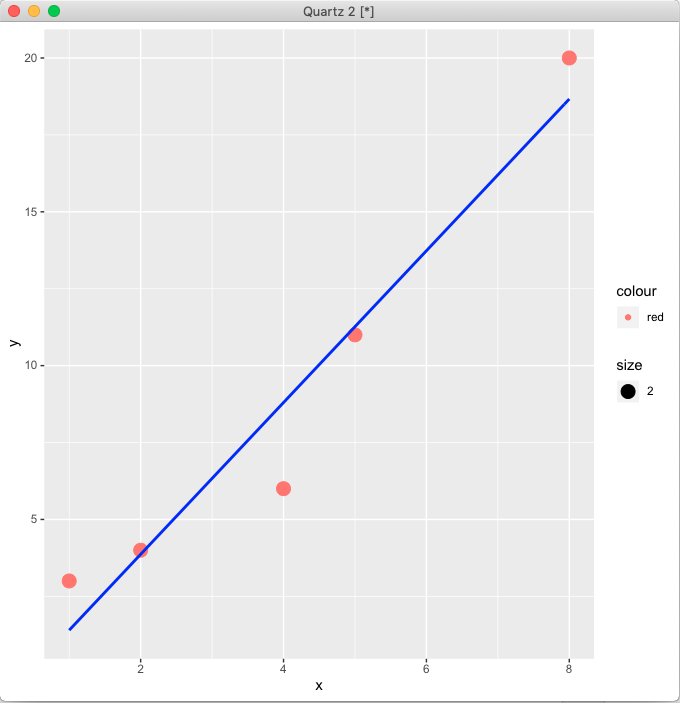
\includegraphics[width = .7\textwidth]{plot1.png} \\

\paragraph{Question Two}
  A rectangular heat storage unit of length $L$, width $W$ and height $H$ will be
  used to store heat energy temporarily. Heat of the unit shall be lost for two
  reasons, by convection and by radiation. The rates of heat loss hc due to
  convection and heat loss hr due to radiation are given respectively by:
  \begin{align*}
    h_c = k_c A(T-T_a) \\
    h_r = k_r A(T^4 - T^4_a)
  \end{align*}
  when $k_c$ and $k_r$ are constants,$T$ is the temperature of the heat storage
  unit, $A$ is the surface area of the unit, and assume that $T$ and $T_a$ are
  constants. The heat energy stored in the unit is given by:
  \begin{align*}
    Q = kV(T - T_a)
  \end{align*}
  where $k$ is a constant and $V$ is the volume of the storage unit. The storage
  unit should have the ability to store at least $Q'$ unit of heat energy
  initially. Furthermore, suppose that space availability restricts the
  dimensions of the storage unit to:
  \begin{align*}
    0 \leq L \leq L', \ 0 \leq W \leq W', \ 0 \leq H \leq H'
  \end{align*}
  Formulate the problem of finding the dimensions $L$,$W$ and $H$ to minimize
  the heat loss in per unit of time.
\paragraph{\color{red}{Answer:}}
In this question, we have to minimize $A$ with those restricts:
\begin{align*}
  &minimize: &A  \\
  &s.t.      &kV(T - T_a) &\geq Q' \\
  &          &V &= LWH \\
  &          &A &= \pi DH + \frac{1}{2}\pi D^2 \\
  &          &0 \leq L \leq L', \ 0 &\leq W \leq W', \ 0 \leq H \leq H'
\end{align*}

\paragraph{Question Three}
Formulate the model in the last exercise if the storage unit is a cylinder of
diameter $D$ and height $H$.

\paragraph{\color{red}{Answer:}}
Since we have to minimize $h_c + h_r$ and $K, T \text{ and } T_a$ are constants,
so we can get this equation:
\begin{align*}
  &minimize: &A  \\
  &s.t.      &kV(T - T_a) &\geq Q' \\
  &          &V &= LWH \\
  &          &A &= \pi DH + \frac{1}{2}\pi D^2 \\
  &          &0 \leq L \leq L', \ 0 &\leq W \leq W', \ 0 \leq H \leq H'
\end{align*}

\paragraph{Question Four}
  An office room of length $60$ meters and width $35$ meters is to be illuminated
  by $16$ light bulbs of wattage $W_i,(i \in(1,\dots,16))$. THe bulbs are to be
  located $2$ meters above the working surface. Let $(x_i, y_i)$ denote the $x$
  and $y$ coordinates of the $ith$ bulb. To ensure lighting, illmination is
  checked at the working surface level at grid points of the form $ (\alpha, \beta)$,
   where:
  \begin{align*}
    \alpha &= 10p, \ p = 0,1,2,\dots,6\\
    \beta &= 5q, \ q = 0,1,\dots, 7
  \end{align*}
     The illumination at $(\alpha, \beta)$ resulting from a bulb of wattage $W_i$
     located at $(x_i, y_i)$ is given by:
  \begin{align*}
    E_i(\alpha, \beta) = k \frac{W_i \parallel(\alpha,\beta) - (x_i, y_i)\parallel}
    {\parallel(\alpha,\beta,2) - (x_i, y_i,0)\parallel^3} \\
  \end{align*}
  when $k$ is a constant reflecting the efficiency of the bulb. The total illumination
  at $(\alpha, \beta)$ is equal to $\displaystyle \sum^6_{i=1}E_i(\alpha, \beta)$. At each of
  the points checked, an illumination of between $2.6$ and $3.2$ units is required.
  All bulbs have same wattage, say $w$, and assume that the wattage $w$ may be chosen
  as any value between $40W, 200W$. Formulate a model to decide a minimum wattage $w$
  for the $16$ bulbs so that the lighting requirement is met.

\paragraph{\color{red}{Answer:}}
  According to the question, we need to minimize the $w$: \\
\begin{align*}
  &minimize: &w  \\
  &s.t.      &2.6 \leq k\frac{W_i \parallel(\alpha,\beta) - (x_i, y_i)\parallel}{\parallel(\alpha,\beta,2) - (x_i, y_i,0)\parallel^3} \leq 3.2 \\
  &          &40 \leq w \leq 200, where i \in (1,2,\dots,6)
\end{align*}

\paragraph{Question Five}
  For the above Problem $4$, now assume that the wattage $w$ for the 16 bulbs
  has only four possible choices: $40W,60W,100W \text{ and } 200W$. How would
  you revise the model?

\paragraph{\color{red}{Answer:}}
  According to the question, we need to minimize the $w$: \\
\begin{align*}
  &minimize:  &w  \\
  &s.t.       &2.6 \leq k\frac{W_i \parallel(\alpha,\beta) - (x_i, y_i)\parallel}{\parallel(\alpha,\beta,2) - (x_i, y_i,0)\parallel^3} \leq 3.2 \\
  &           &w = 40k_1 + 60k_2 + 100k_3 + 200k_4 \\
  &           &k_1 + k_2 + k_3 + k_4 =1, \ where i \in (1,2,\dots,16)\\
  &           &\text{$k_1, k_2, k_3$ and $k_4$ are $0 - 1$ variables} \\
\end{align*}

\paragraph{Question Six}
  Return to Problem $4$ Assume it is decided that all bulbs used have the wattage
  $100W$, but we want to use the least number of bulbs to meet the lighting request.
  It is known that $16$ such bulbs are enough, but we wish to use as few bulbs as
  possible. Give a model to determine how many bulbs are required and where
  should they be located.

\paragraph{\color{red}{Answer:}}
  we can notice that: \\
  \begin{align*}
    x_i = ap',\ p &= 0,1,\dots \frac{60}{a} \\
    y_i = bq',\ q &= 0,1,\dots \frac{35}{b},\\
    where \ i &= 1,2,\dots, \frac{(60 + a)(35 + b)}{ab}
  \end{align*}
\textbf{a} is the interval of the bulbs along the length of the office room while
\textbf{b} is the width of the room. So, we can get the optimal equation: \\
\begin{align*}
  &minimize:  &\frac{(60 + a)(35 + b)}{ab}  \\
  &s.t.       &2.6 \leq k\frac{W_i \parallel(\alpha,\beta) - (x_i, y_i)\parallel}{\parallel(\alpha,\beta,2) - (x_i, y_i,0)\parallel^3} \leq 3.2 \\
  &           &w = 100 \\
\end{align*}


\end{document}
